

\section{Task IV : Great Coach Effect}

\subsection{Problem Analysis}
It's not easy for athletes to serve in teams of different nations, but coaches can\cite{thompson2016analyzing}

Two possible examples of this include Lang Ping,
who coached volleyball teams from both the U.S. and China to championships, and the
sometimes-controversial gymnastics coach, Béla Károlyi, who coached Romania and
then the U.S. women's teams with great success. \cite{2,3}

Bela and Marta instructed the US gym team in the following years:

1981: They defected to the US and began coaching gymnastics soon after.

1984: They coached Mary Lou Retton, who won America's first gold medal in the Olympic all - arounds.

1991: They trained Kim Zmeskal, who became the world champion.

1996: Marta coached the "Magnificent Seven" member Kerri Strug to win the Olympic team gold.

2000: Bela was named national team coordinator.

2001 - 2016: Marta served as the coordinator of the US women's gymnastics national team.

Since there's too little data of Lang Ping, we decide to use Bela and Marta as an example to train data. We use comprehensive methods developed by previous tasks and establish the last part of our \textbf{`PRE'} model : \textbf{Legendary Index} .

To find out coaches influence on some achievements of certain countries in the history, we define \textbf{Legendary Index}, representing the greatness of a country's achievement during a certain period.
Then, by analyzing those with a high \textbf{Legendary Index}, we can find out the impact of \textbf{Great Coaches}.

\subsection{Model Establishment : Legendary Index}
We rearrange the data by Sport, NOC, and Sex. 

Since we do not have specific information on which events or disciplines Bela and Marta coached, we only consider sports, gender, and country. We assign a value of 1 if a great coach is coaching and 0 if not.Then we split the data into training, testing dataset and train our model by year according to specific parameters.Finally, We use the model to calculate Legendary Index to indicate greatness.\cite{johnson2022machine}

\begin{lstlisting}[caption=Part of the Model]
from sklearn.model_selection import train_test_split
from sklearn.metrics import mean_squared_error
from sklearn.ensemble import RandomForestRegressor
import xgboost as xgb
from sklearn.tree import DecisionTreeRegressor
from sklearn.metrics import accuracy_score
legendary_years 
= [1976, 1981, 1984, 1989, 1996, 2000, 2004, 2008, 2012, 2016, 2020]
us_women_gymnastics.loc[:, 'Legendary_Coach'] 
= us_women_gymnastics['Year'].apply(lambda x: 1 if x in legendary_years else 0)
    ...
params = {
    'objective': 'reg:squarederror',
    'learning_rate': 0.01,
    'max_depth': 6,
    'min_child_weight': 1,
    'subsample': 0.8,
    'colsample_bytree': 0.8,
    'n_estimators': 1000,
    'random_state': 42,
    'early_stopping_rounds': 10
}

model = xgb.XGBRegressor(**params)
model.fit(X_train, y_train,
          eval_set=[(X_train, y_train), (X_test, y_test)], 
          verbose=False) 
          ...
          medal_counts0 = group.groupby('Year')['Medal'].value_counts().unstack(fill_value=0)
          medal_counts0 = medal_counts0.reindex(columns=['Gold', 'Silver', 'Bronze', 'No medal'], fill_value=0)
          medal_counts0['Total'] = medal_counts0[['Gold', 'Silver', 'Bronze']].sum(axis=1)
          medal_counts0 = medal_counts0[['Total', 'Gold', 'Silver', 'Bronze', 'No medal']].reset_index()
         
          medal_counts0 = medal_counts0.reset_index()
          
          medal_counts0['Sport'] = sport
          medal_counts0['NOC'] = noc
          medal_counts0['Sex'] = sex
          
legendary_coach_results = pd.DataFrame()

    for (sport, noc, sex), group in grouped_all_medal_counts:
        group['Legendary_Index'] = model.predict(group[['Year', 'Total', 'Gold', 'Silver', 'Bronze', 'No medal']])
              
        legendary_threshold = 0.68
            
        group['Predicted_Legendary_Coach'] = group['Legendary_Index'] > legendary_threshold
              
        result = group[['Year','Sport', 'NOC', 'Sex', 'Legendary_Index', 'Predicted_Legendary_Coach']]
          
\end{lstlisting}

Part of the calculation is in \textbf{Figure \ref{fig:legendary_index_detailed}}.

This is the real calculation formula behind the code\cite{miller2020comparative}:
\begin{center}
$ x = [\textit{`Year'}, \textit{`Total'}, \textit{`Gold'}, \textit{`Silver'}, \textit{`Bronze'}, \textit{`No medal'}]$

$\hat{y} = \sum_{k=1}^{K} \alpha_k h_k(x)$

$L(\theta) = \sum_{i=1}^{n} \left( y_i - \hat{y}_i \right)^2 + \sum_{k=1}^{K} \left( \gamma T_k + \frac{1}{2} \lambda \sum_{j=1}^{T_k} w_{kj}^2 \right)$

\end{center}

Because of the limitation of the data of Bela and Marta, we can't get a very accurate Legendary Index. But it can still serve as indication of greatness.

\begin{figure}[h]
\centering
    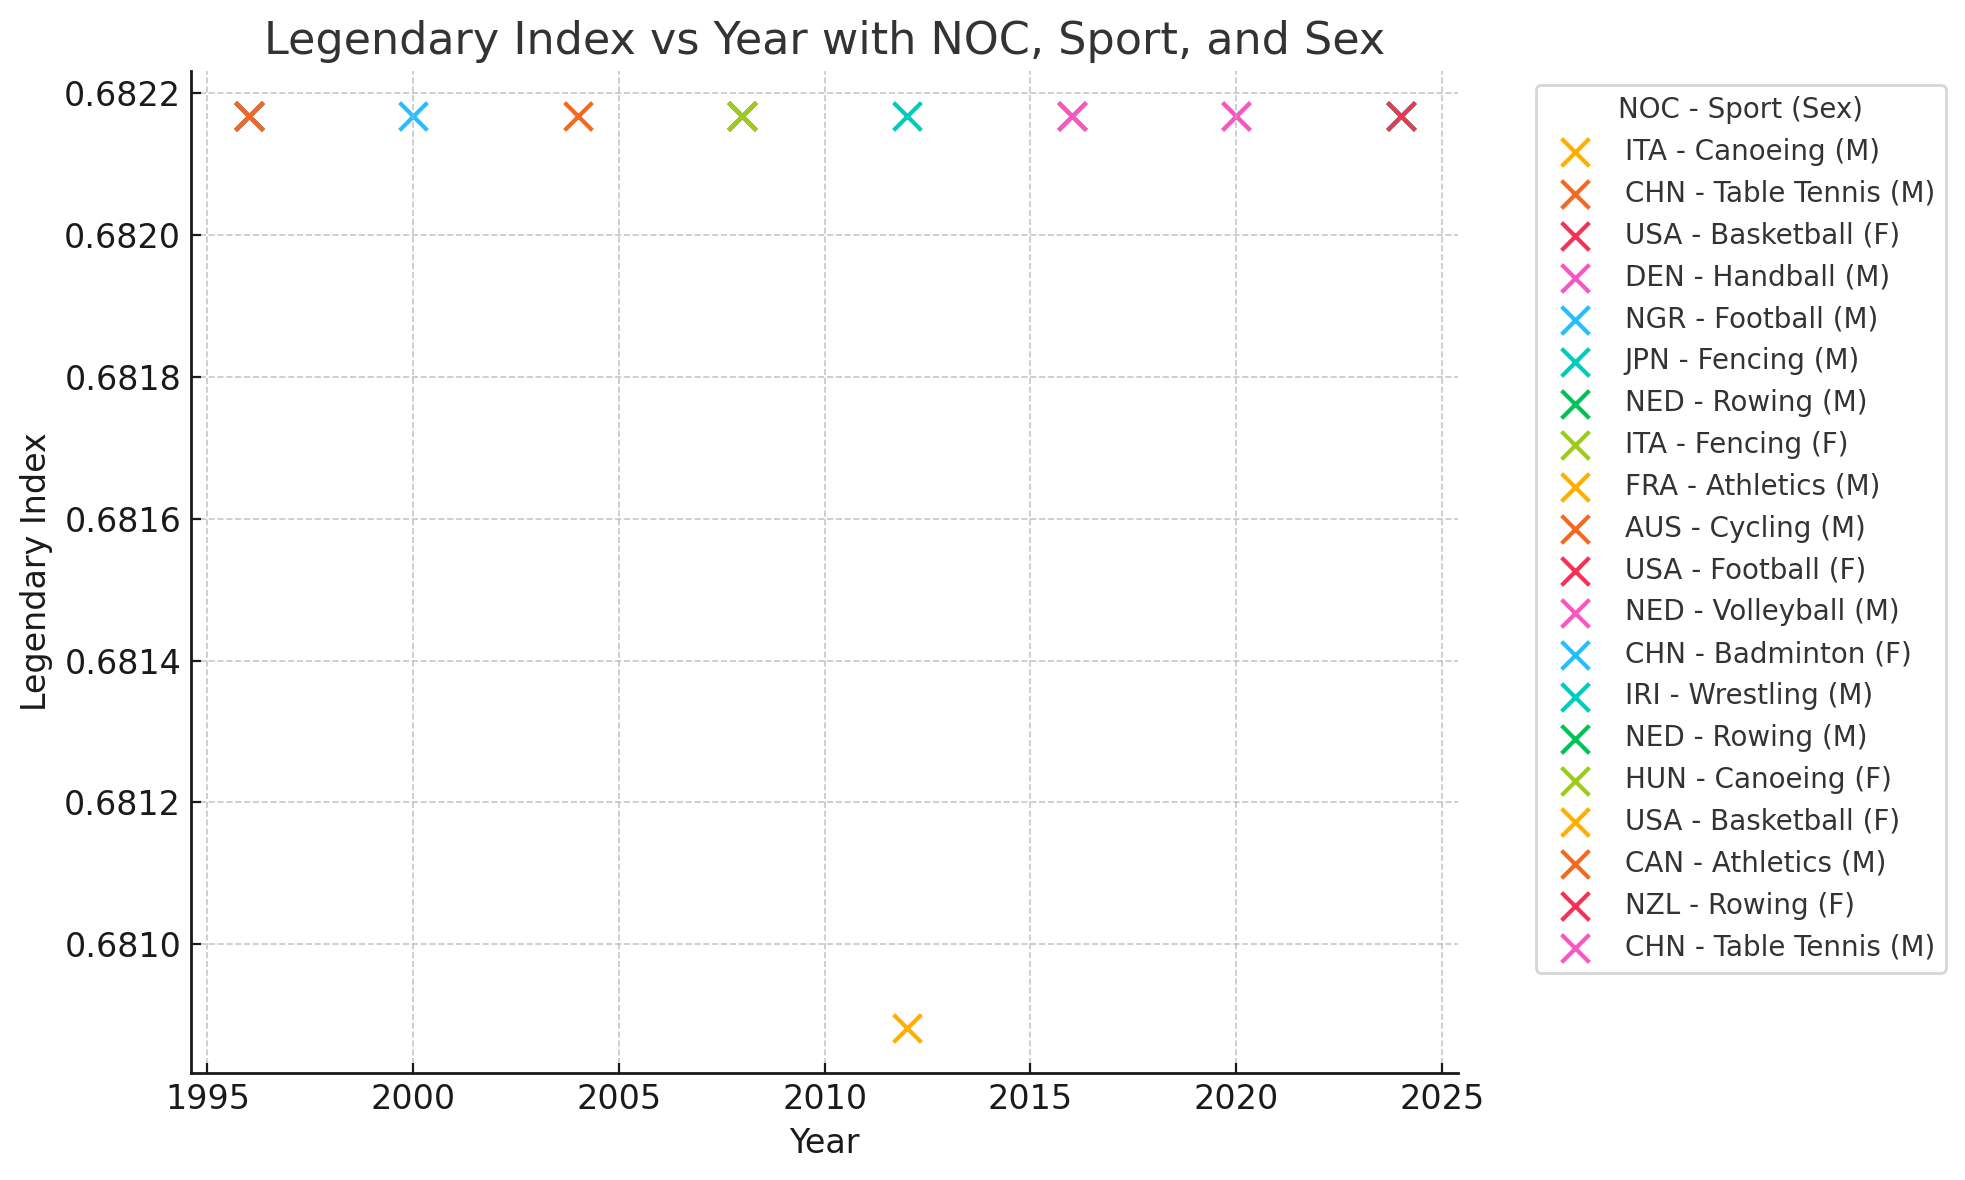
\includegraphics[width=1\textwidth]{./figures/Lengendary_index_detailed.png}
    \caption{Legendary Index of certain events}
    \label{fig:legendary_index_detailed}
\end{figure}

\subsection{Lang Ping: The Great Coach}

Fortunately, We've found Lang Ping in the Predicted Great Coach.

\begin{figure}[h]
    \centering
    \begin{subfigure}[b]{0.32\textwidth}
        \centering
        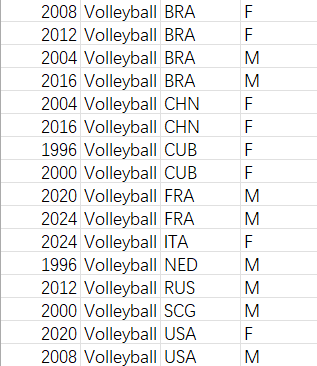
\includegraphics[width=\textwidth]{../figures/lang_ping.png}
        \caption{Lang Ping: The Great Coach}
        \label{fig:lang_ping1}
    \end{subfigure}
    \begin{subfigure}[b]{0.32\textwidth}
        \centering
        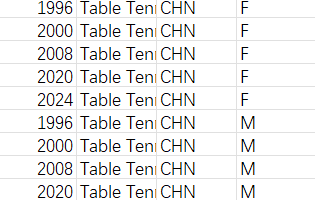
\includegraphics[width=\textwidth]{../figures/chn_tt.png}
        \caption{Chinese Table Tennis}
        \label{fig:chn_tt}
    \end{subfigure}
    \begin{subfigure}[b]{0.32\textwidth}
        \centering
        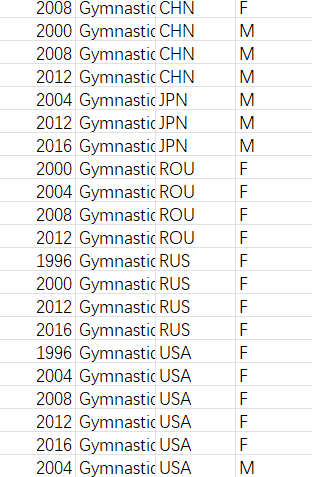
\includegraphics[width=\textwidth]{../figures/gym.png}
        \caption{Gymnastics}
        \label{fig:gym}
    \end{subfigure}
    \caption{Great Achievements Detected}
    \label{fig:lang_ping_combined}
\end{figure}

Besides Lang Ping, other great achievements are also detected. Although we don't have enough time to check every achievements with the information of the internet, every data we have checked is really great achievement.

Shown in \textbf{Figure \ref{fig:lang_ping_combined}}, Chinese Table Tennis and Gymnastics are selected as the most famous examples. 1996, 2000, 2008 and 2020 are great years for Chinese Male Table Tennis team, while 2024 is not although they got the gold medal.

We've even found interesting data of controversial results caused by the penalty awarded by referee.In 2024, Italy fencing is very close to greatness, and they've complained about the referee's decision.\cite{4}

Coach of 2024 US female football team Emma Hayes is considered as great coach according to our model.She was named The Best FIFA Women's Coach of 2024.\cite{5}

\subsection{Three Countries to invest in `great' coach}

From the data, three countries will benefit a lot from investing a 'great' coach.

China Table Tennis Male 2024 : With rather great achievement, Chinese table tennis team is close to greatness.However, it's not enough compared to it's past glory.Maybe changing the current coach is a good choice.

Korea Judo Male and Female 2024 : As a key event of Korea, it's not enough for them to stop their step. A great coach may lead them to greated achievements.

India Badminton Female 2024 : Only great athletes are not enough. They need great coach to fully show their potential. Although they are already creating new history, a great coach can lift them to higher places.

There're many Countries and Sports that need great coaches. Only three asian countries are chosen as examples to show that  great coach effect may help on different situation.

Besides, using the Legendary Index of our model, it's easier to discover potential great teams and athletes.We will discuss it's further application next chapter.
